\subsection{Sơ đồ thực thể mối quan hệ}
\label{subsec:db_erd}

Một ERD chứa toàn bộ bảng cache sẽ trải dài theo chiều ngang và che khuất các quan hệ quan trọng. Báo cáo vì vậy dùng ba lát cắt bên cạnh sơ đồ tổng quan. Mỗi hình giữ khóa chính, khóa ngoại và một số cột đại diện. Đường liền biểu diễn quan hệ khóa ngoại; đường nét đứt biểu diễn liên hệ logic bằng address hoặc signature. Một số hộp như \texttt{USER\_WALLET\_DATA}, \texttt{TOKEN\_MARKET\_CHART} và \texttt{WALLET\_ENHANCED\_DETAILS} đại diện cho một nhóm bảng vật lý có cùng vai trò.

\begin{figure}[H]
    \centering
    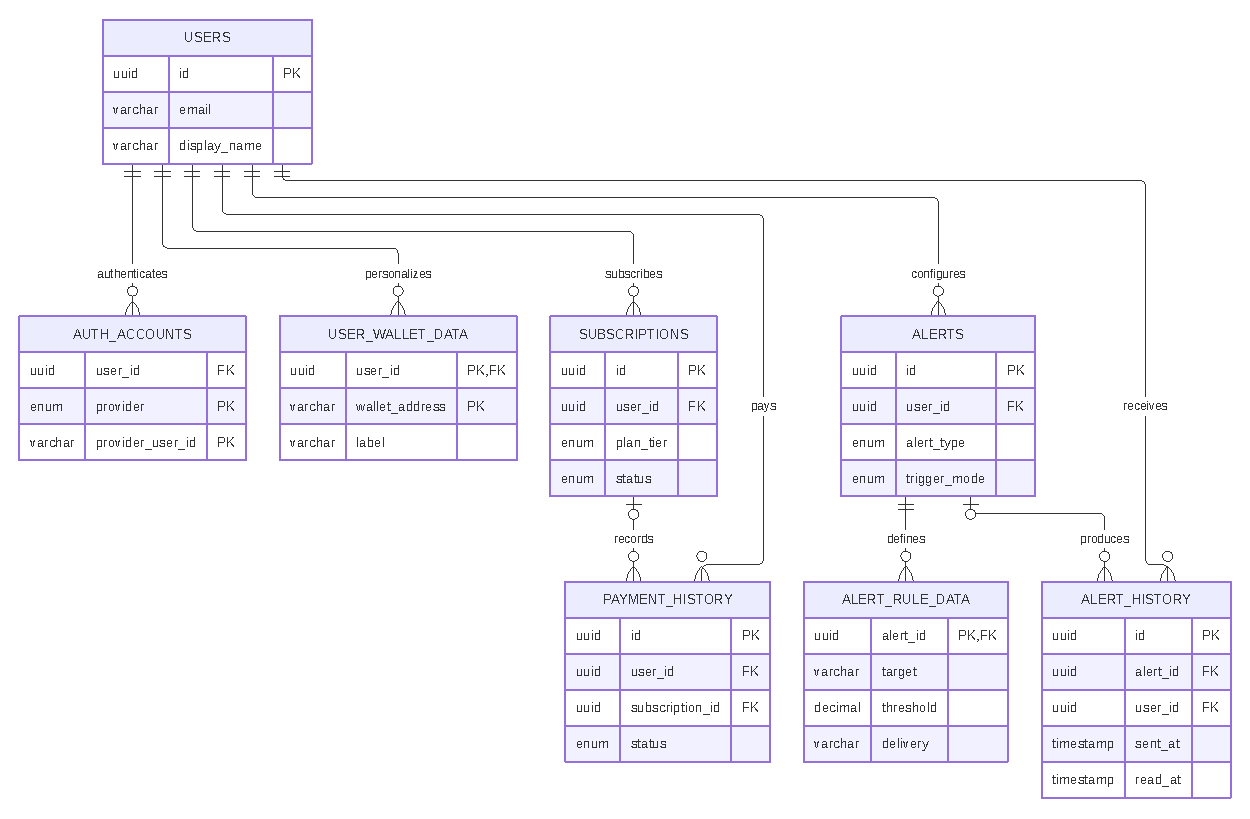
\includegraphics[width=0.98\textwidth,height=0.72\textheight,keepaspectratio]{Chapter3/diagrams/identity-alert.pdf}
    \caption{ERD nhóm tài khoản, thanh toán và cảnh báo}
    \label{fig:db_identity_alert}
\end{figure}

Hình~\ref{fig:db_identity_alert} đặt \texttt{users} ở gốc của dữ liệu có tính sở hữu. Tài khoản có thể liên kết nhiều phương thức xác thực và ví, đồng thời sở hữu subscription, lịch sử thanh toán và cấu hình cảnh báo. Cấu hình cảnh báo được tách khỏi lịch sử phát sinh để người dùng có thể thay đổi rule mà vẫn giữ các thông báo đã nhận và trạng thái đọc.

\begin{figure}[H]
    \centering
    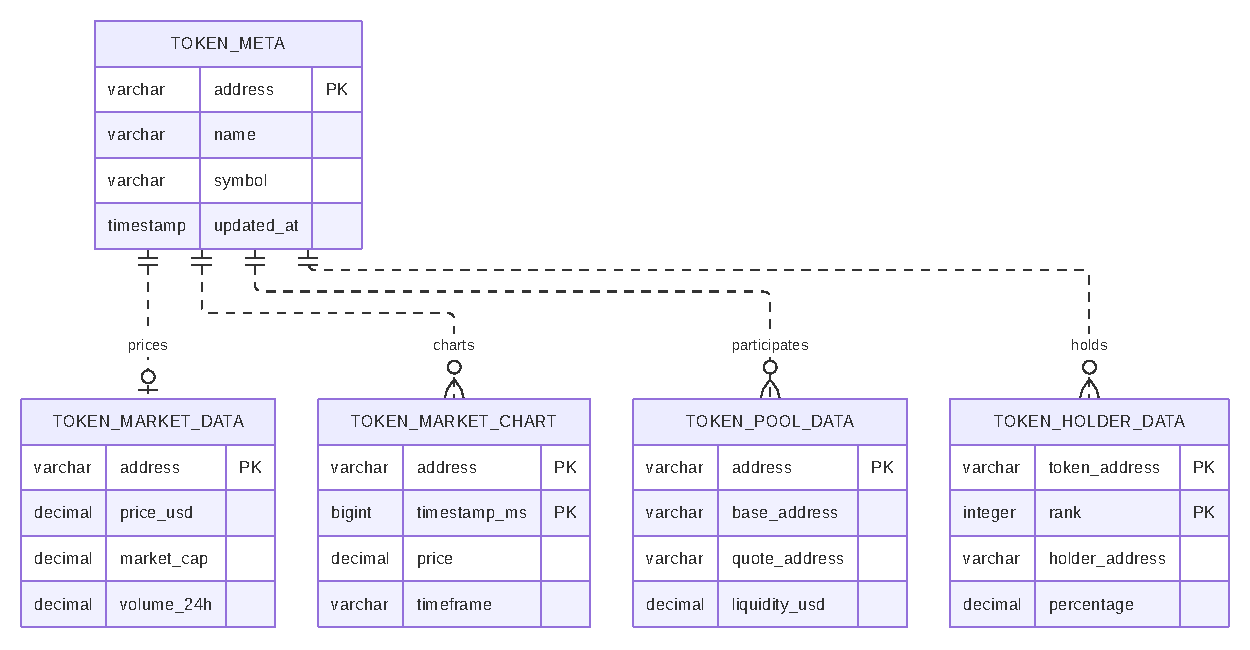
\includegraphics[width=0.96\textwidth]{Chapter3/diagrams/token-market-panel.pdf}

    \vspace{0.5em}
    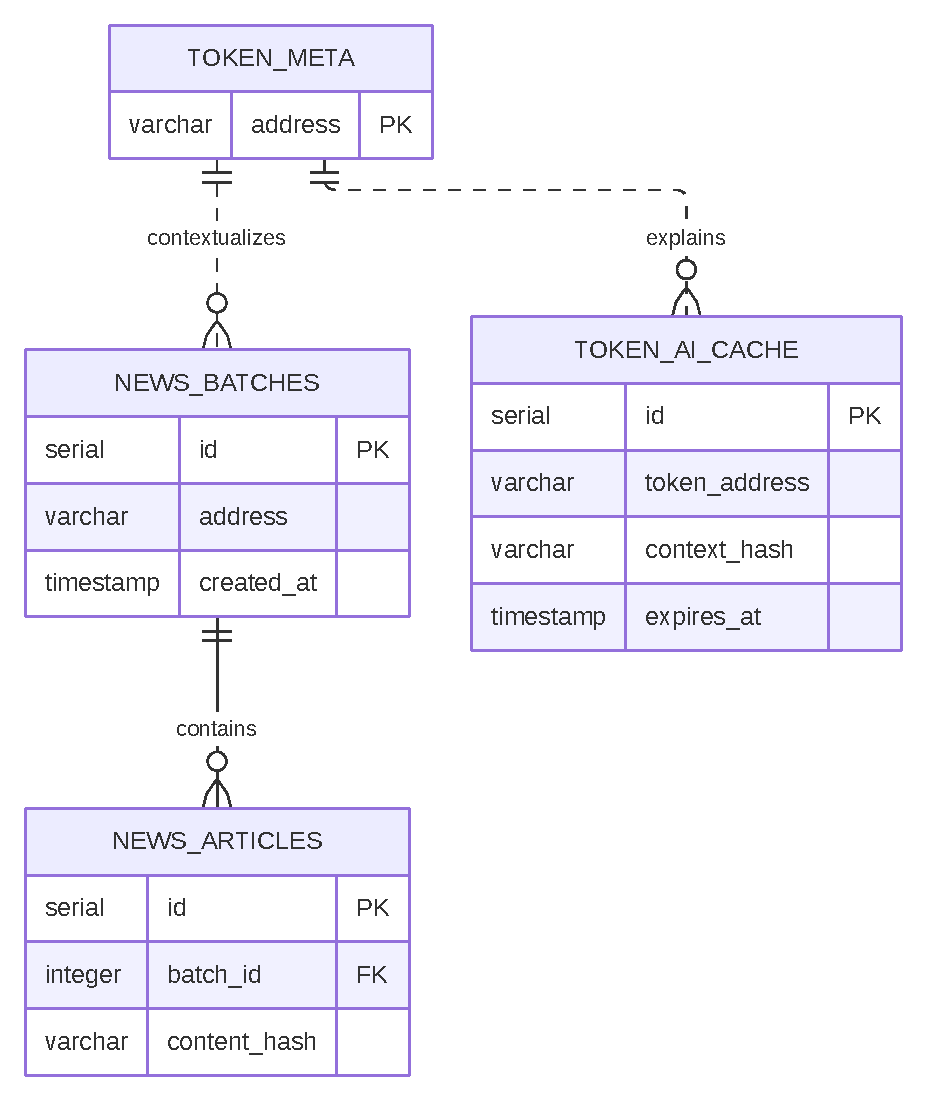
\includegraphics[width=0.62\textwidth,height=0.34\textheight,keepaspectratio]{Chapter3/diagrams/token-content-panel.pdf}
    \caption{ERD nhóm token, thị trường, pool và nội dung phân tích}
    \label{fig:db_token_data}
\end{figure}

Hình~\ref{fig:db_token_data} sử dụng token address làm điểm nối logic. Metadata, market snapshot, chuỗi giá, pool và holder được tách vì có nguồn và chu kỳ cập nhật khác nhau. News được tổ chức thành batch và article bằng khóa ngoại; cache AI liên kết với token bằng address và context hash để tái sử dụng câu trả lời trong cùng ngữ cảnh.

\begin{figure}[H]
    \centering
    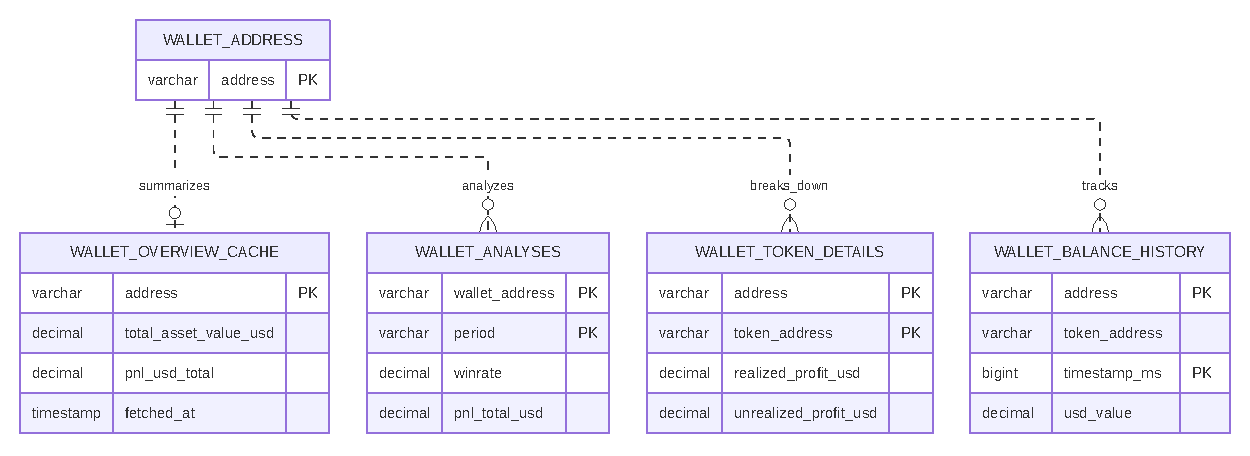
\includegraphics[width=0.96\textwidth]{Chapter3/diagrams/wallet-analysis-panel.pdf}

    \vspace{0.5em}
    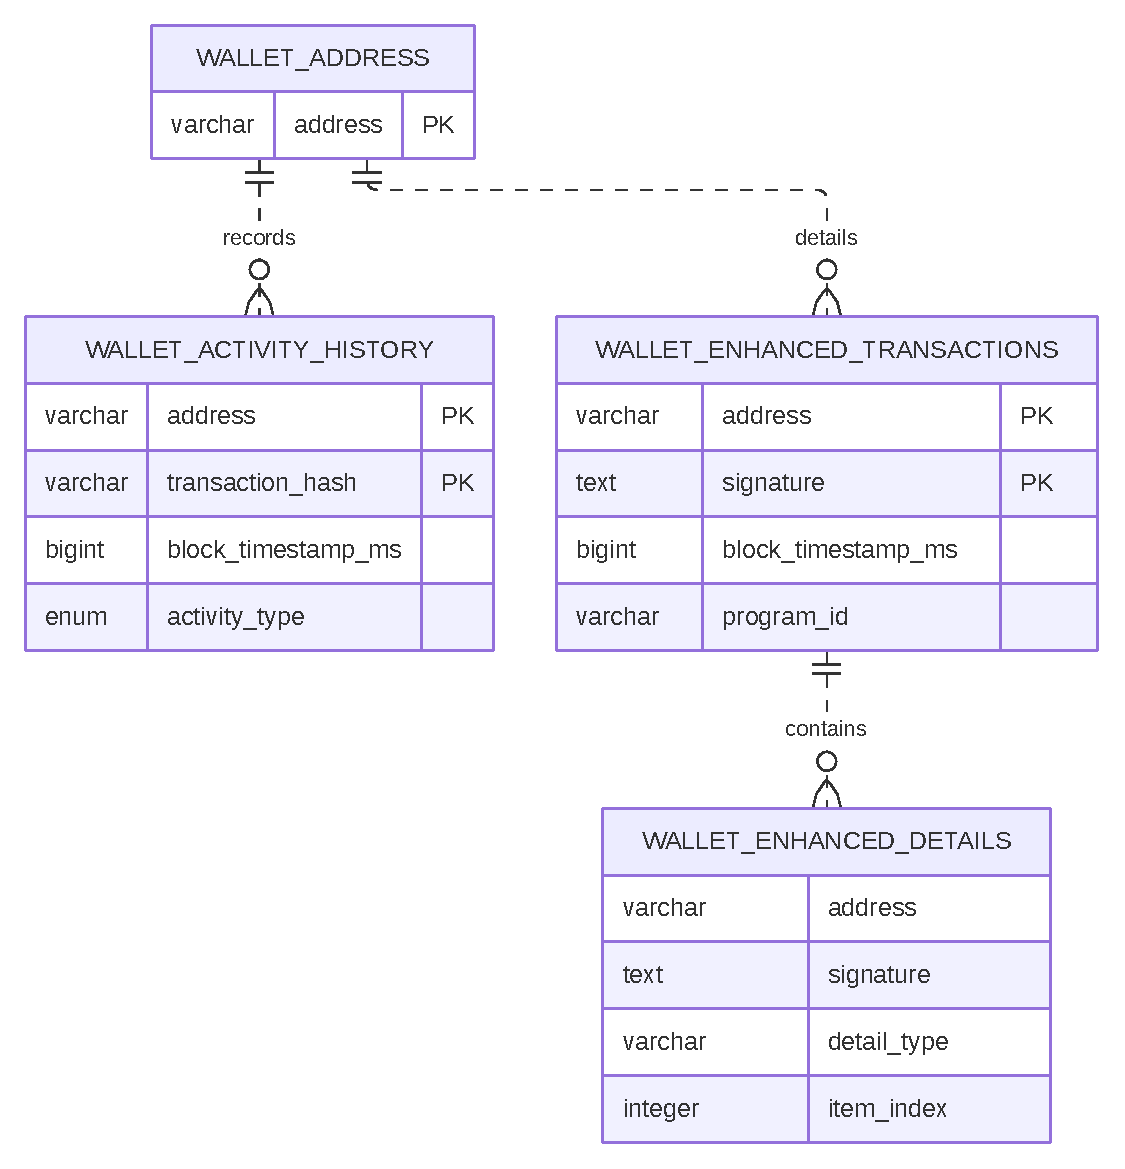
\includegraphics[width=0.58\textwidth,height=0.36\textheight,keepaspectratio]{Chapter3/diagrams/wallet-activity-panel.pdf}
    \caption{ERD nhóm ví, lịch sử giao dịch và kết quả phân tích}
    \label{fig:db_wallet_data}
\end{figure}

Hình~\ref{fig:db_wallet_data} dùng \texttt{WALLET\_ADDRESS} như một thực thể logic. Overview cache cung cấp dữ liệu tổng hợp cho lần mở trang đầu tiên; bảng phân tích lưu PnL, win rate và phân rã theo token cho từng kỳ; các bảng lịch sử giữ số dư và hoạt động swap/transfer theo thời gian. Enhanced transaction liên kết với các dòng chi tiết bằng address và signature, phục vụ khi người dùng mở một giao dịch để xem transfer, instruction và chương trình liên quan.
